%%**************************************************************
%% Vorlage fuer Bachelorarbeiten (o.ä.) der DHBW
%%
%% Autor: Tobias Dreher, Yves Fischer
%% Datum: 06.07.2011
%%
%% Autor: Michael Gruben
%% Datum: 15.05.2013
%%**************************************************************

%!TEX root = ../dokumentation.tex       

\documentclass[%
	pdftex,
	oneside,		% Einseitiger Druck.
	12pt,			% Schriftgroesse
	parskip=half,	% Halbe Zeile Abstand zwischen Absätzen.
	headsepline,	% Linie nach Kopfzeile.
	footsepline,	% Linie vor Fusszeile.
	abstracton,	    % Abstract Überschriften
	ngerman,		% Translator
]{scrreprt}

\usepackage{geometry}
\geometry{a4paper, top=45mm, left=25mm, right=35mm, bottom=30mm,
headsep=15mm, footskip=20mm}

\usepackage{tocloft}

\renewcommand*\chapterheadstartvskip{\vspace*{-1cm}}

\usepackage[headsepline,plainheadsepline]{scrpage2}
\pagestyle{scrheadings}
\ihead[\rightmark]{\rightmark} \chead[]{}


\automark[chapter]{chapter}
\renewcommand{\chaptermark}[1]{\markright{\ #1}}


\usepackage{wrapfig}

\usepackage{pdfpages}
%Zeilenumbruch und mehr
\usepackage[activate]{microtype}

% Zeichencodierung
\usepackage[utf8]{inputenc}
\usepackage[T1]{fontenc}

% Zeilenabstand
\usepackage[onehalfspacing]{setspace}

% Index-Erstellung
\usepackage{makeidx}

% Lokalisierung (neue deutsche Rechtschreibung)
\usepackage[ngerman]{babel}

% Anführungszeichen 
\usepackage[babel,german=quotes]{csquotes}
%\usepackage[style=swiss]{csquotes}


% Spezielle Tabellenform fuer Deckblatt
\usepackage{longtable}
\setlength{\tabcolsep}{10pt} %Abstand zwischen Spalten
\renewcommand{\arraystretch}{1.5} %Zeilenabstand

% Grafiken
\usepackage{graphicx}

% Mathematische Textsaetze
\usepackage{amsmath}
\usepackage{amssymb}

% Pakete um Textteile drehen zu können, oder eine Seite Querformat anzeigen kann.
%\usepackage{rotating}
%\usepackage{lscape}

% Farben
\usepackage{color}
\definecolor{LinkColor}{rgb}{0,0,0}
\definecolor{ListingBackground}{rgb}{0.92,0.92,0.92}

\newcommand{\pdftitel}{Dokumentation zum Unternehmensplanspiel "Avalon"}
\newcommand{\autor}{Johannes Haaß}
\newcommand{\arbeit}{Seminararbeit}

% Titel, Autor und Datum
\title{\titel}
\author{\autor}
\date{\datum}

% PDF Einstellungen
\usepackage[%
	pdftitle={\pdftitel},
	pdfauthor={\autor},
	pdfsubject={\arbeit},
	pdfcreator={pdflatex, LaTeX with KOMA-Script},
	pdfpagemode=UseOutlines, % Beim Oeffnen Inhaltsverzeichnis anzeigen
	pdfdisplaydoctitle=true, % Dokumenttitel statt Dateiname anzeigen.
	pdflang=de % Sprache des Dokuments.
]{hyperref} 

% (Farb-)einstellungen für die Links im PDF
\hypersetup{%
	colorlinks=true, % Aktivieren von farbigen Links im Dokument
	linkcolor=LinkColor, % Farbe festlegen
	citecolor=LinkColor,
	filecolor=LinkColor,
	menucolor=LinkColor,
	urlcolor=LinkColor,
	bookmarksnumbered=true % Überschriftsnummerierung im PDF Inhalt anzeigen.
}

% Literaturverweise nach Harvard (mit deutschem und)
\usepackage[dcucite]{harvard}
\renewcommand{\harvardand}{und}
\renewcommand{\harvardurl}{URL: \url}


% Verschiedene Schriftarten
%\usepackage{goudysans}
%\usepackage{lmodern}
\usepackage{url} 
%\usepackage{libertine}
\usepackage{palatino} 

% Hurenkinder und Schusterjungen verhindern
% http://projekte.dante.de/DanteFAQ/Silbentrennung
\clubpenalty=10000
\widowpenalty=10000
\displaywidowpenalty=10000



% Quellcode
\usepackage{listings}
\lstloadlanguages{bash}
\lstset{language=bash}
\lstset{%
	%language=PHP,		 	 % Sprache des Quellcodes
	numbers=left,           % Zelennummern links
	stepnumber=1,            % Jede Zeile nummerieren.
	numbersep=5pt,           % 5pt Abstand zum Quellcode
	numberstyle=\tiny,       % Zeichengrösse 'tiny' für die Nummern.
	breaklines=true,         % Zeilen umbrechen wenn notwendig.
	breakautoindent=true,    % Nach dem Zeilenumbruch Zeile einrücken.
	postbreak=\space,        % Bei Leerzeichen umbrechen.
	tabsize=2,               % Tabulatorgrösse 2
	basicstyle=\ttfamily\footnotesize, % Nichtproportionale Schrift, klein für den Quellcode
	showspaces=false,        % Leerzeichen nicht anzeigen.
	showstringspaces=false,  % Leerzeichen auch in Strings ('') nicht anzeigen.
	extendedchars=true,      % Alle Zeichen vom Latin1 Zeichensatz anzeigen.
	captionpos=b,            % sets the caption-position to bottom
	backgroundcolor=\color{ListingBackground} % Hintergrundfarbe des Quellcodes setzen.
}
%%%% so einbinden ------> \lstinputlisting{quellcode/2.abap}

% Glossar
\usepackage[
	nonumberlist, %keine Seitenzahlen anzeigen
	%acronym,      %ein Abkürzungsverzeichnis erstellen
	%section,     %im Inhaltsverzeichnis auf section-Ebene erscheinen
	toc,          %Einträge im Inhaltsverzeichnis
]{glossaries}

%Akronyme
\usepackage[printonlyused,footnote]{acronym}

% Fussnoten
\usepackage[perpage, hang, multiple, stable]{footmisc}

%Bildpfad
\graphicspath{{images/}}

%nur ein latex-Durchlauf für die Aktualisierung von Verzeichnissen nötig
\usepackage{bookmark}

%Gleitumgebungen (Bilder, Tabellen, usw\ldots) lassen sich mit H an genau der
% definierten Stelle platzieren
\usepackage{float}

% für die vertikale Platzierung von Text in Tabellen
\usepackage{array}

% für die Darstellung des Euro-Symbols
\usepackage[right]{eurosym}

% für textumflossene Grafiken
\usepackage{wrapfig}

% eine Kommentarumgebung "k" (Handhabe mit \begin{k}<Kommentartext>\end{k},
% Kommentare werden rot gedruckt). Wird \% vor excludecomment{k} entfernt,
% werden keine Kommentare mehr gedruckt.
\usepackage{comment}
\specialcomment{k}{\begingroup\color{red}}{\endgroup}
%\excludecomment{k}


% Ab jetzt können auch Umlaute verwendet werden

%falls pdftitel = titel der Arbeit
\newcommand{\titel}{\pdftitel}
%bei unterschiedlichen Titeln
%\newcommand{\titel}{In der Regel haben wir einen zweizeiligen
% Bachelorthesistitel}
\newcommand{\martrikelnr}{1234567}
\newcommand{\kurs}{WI SE B 2012}
\newcommand{\datumAbgabe}{August 2012}
\newcommand{\firma}{Firma GmbH}
\newcommand{\firmenort}{Firmenort}
\newcommand{\abgabeort}{Abgabeort}
\newcommand{\abschluss}{Bachelor of Engineering}
\newcommand{\studiengang}{Studienganges Vorderasiatische Archäologie}
\newcommand{\dhbw}{Stuttgart Campus Horb}
\newcommand{\betreuer}{Dipl.-Ing. (FH) Peter Pan}
\newcommand{\gutachter}{Dr. Silvana Koch-Mehrin}
\newcommand{\zeitraum}{12 Wochen}
\newcommand{\arbeitsart}{\arbeit}

\makeglossaries
%!TEX root = ../dokumentation.tex

%
% vorher in Konsole folgendes aufrufen: 
%	makeglossaries makeglossaries dokumentation.acn && makeglossaries dokumentation.glo
%

%
% Glossareintraege --> referenz, name, beschreibung
% Aufruf mit \gls{...}
%
\newglossaryentry{Glossareintrag}{name={Glossareintrag},plural={Glossareinträge},description={Ein Glossar beschreibt verschiedenste Dinge in kurzen Worten}}


\begin{document}

	% Deckblatt
	\begin{spacing}{1}
		%!TEX root = ../dokumentation.tex

\begin{titlepage}
	\begin{longtable}{p{.4\textwidth} p{.4\textwidth}}
	  {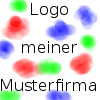
\includegraphics[height=2.6cm]{images/logo.png}} & 
	  {
\includegraphics[height=2.6cm]{images/dhbw.png}}
	\end{longtable}
	\enlargethispage{20mm}
	\begin{center}
	 \vspace*{0mm} Duale Hochschule Baden-Württemberg \\ \dhbw\\
	 	\vspace*{10mm}	{\large\bf \arbeit}\\
	 	  \vspace*{12mm}	{\LARGE\bf \titel }\\
	 	  
	 	  \vspace*{12mm}	\studiengang\\
	 	  
	 	  \vspace*{5mm}	\zeitraum\\
	\end{center}
	\vfill
	\begin{spacing}{1}
	\begin{tabbing}
		mmmmmmmmmmmmmmmmmmmmmmmmmm     \= \kill
		\textbf{Verfasser}		\> Martin Achenbach\\
								\> Jonas Braun\\
								\> Johannes Haaß\\
								\> Frederik Pahde\\
		\\
		\textbf{Kurs}  					\> \kurs\\
		\textbf{Studiengangsleiter}	   \>	\studiengangsleiter\\
		\\
		\textbf{Ausbildungsfirma}      \>  \firma\\
									\> Dietmar-Hopp-Allee 16\\
									\> \firmenort\\
									\\
		\textbf{Dozent}              \>  \betreuer \\
									%	\>\betreuermail\\
										\\
		%\textbf{Wissenschaftlicher Betreuer}             \>  \gutachter \\
			%							\>\gutachtermail\\
										  %\vspace*{3mm} 	{\large\bf \autor}\\
	\end{tabbing}
	\end{spacing}
\end{titlepage}

	\end{spacing}
	\newpage

	\renewcommand{\thepage}{\Roman{page}}
	\setcounter{page}{1}

	% Sperrvermerk
	%!TEX root = ../dokumentation.tex

\thispagestyle{empty}
% Sperrvermerk direkt hinter Titelseite
\section*{Sperrvermerk}

\vspace*{2em}

Die vorliegende {\arbeitsart} mit dem Titel {\itshape \titel} ist mit einem Sperrvermerk versehen und wird ausschließlich zu Prüfungszwecken am Studiengang {\studiengang} der Dualen Hochschule Baden-Württemberg {\abgabeort} vorgelegt.
Jede Einsichtnahme und Veröffentlichung – auch von Teilen der Arbeit – bedarf der vorherigen Zustimmung durch die {\firma}.

	\newpage
	
	% Erklärung
	%!TEX root = ../dokumentation.tex

\thispagestyle{empty}

\section*{Erklärung}
% http://www.se.dhbw-mannheim.de/fileadmin/ms/wi/dl_swm/dhbw-ma-wi-organisation-bewertung-bachelorarbeit-v2-00.pdf
\vspace*{2em}

Ich erkläre hiermit ehrenwörtlich: \\
\begin{enumerate}
\item dass ich meine {\arbeitsart} mit dem Thema
{\itshape \titel } ohne fremde Hilfe angefertigt habe;
\item dass ich die Übernahme wörtlicher Zitate aus der Literatur sowie die Verwendung der Gedanken
anderer Autoren an den entsprechenden Stellen innerhalb der Arbeit gekennzeichnet habe;
\item dass ich meine {\arbeitsart} bei keiner anderen Prüfung vorgelegt habe;
\item dass die eingereichte elektronische Fassung exakt mit der eingereichten schriftlichen Fassung
übereinstimmt.
\end{enumerate}

Ich bin mir bewusst, dass eine falsche Erklärung rechtliche Folgen haben wird.

\vspace{3em}

\abgabeort, \datumAbgabe
\vspace{4em}

\autor

	\newpage

	% Abstract
	%!TEX root = ../dokumentation.tex

\pagestyle{empty}

\renewcommand{\abstractname}{Zusammenfassung}
\begin{abstract}
Ein Abstract ist eine prägnante Inhaltsangabe, ein Abriss ohne
Interpretation und Wertung einer wissenschaftlichen Arbeit. In DIN
1426 wird das (oder auch der) Abstract als Kurzreferat zur
Inhaltsangabe beschrieben.

\begin{description}
\item[Objektivität] soll sich jeder persönlichen Wertung enthalten
\item[Kürze] soll so kurz wie möglich sein
\item[Genauigkeit] soll genau die Inhalte und die Meinung der Originalarbeit wiedergeben
\end{description}

Üblicherweise müssen wissenschaftliche Artikel einen Abstract
enthalten, typischerweise von 100-150 Wörtern, ohne Bilder und
Literaturzitate und in einem Absatz.

Quelle \url{http://de.wikipedia.org/wiki/Abstract} Abgerufen 07.07.2011
\end{abstract}


\renewcommand{\abstractname}{Summary}
\begin{abstract}
An abstract is a brief summary of a research article, thesis, review,
conference proceeding or any in-depth analysis of a particular subject
or discipline, and is often used to help the reader quickly ascertain
the paper's purpose. When used, an abstract always appears at the
beginning of a manuscript, acting as the point-of-entry for any given
scientific paper or patent application. Abstracting and indexing
services for various academic disciplines are aimed at compiling a
body of literature for that particular subject.

The terms précis or synopsis are used in some publications to refer to
the same thing that other publications might call an "abstract". In
management reports, an executive summary usually contains more
information (and often more sensitive information) than the abstract
does.

Quelle: \url{http://en.wikipedia.org/wiki/Abstract_(summary)}

\end{abstract}

	\newpage

	\pagestyle{plain}

	% Inhaltsverzeichnis
	\begin{spacing}{1.1}
		\setcounter{tocdepth}{1}
		%für die Anzeige von Unterkapiteln im Inhaltsverzeichnis
		%\setcounter{tocdepth}{2}
		\tableofcontents
	\end{spacing}
	\newpage

	\renewcommand{\thepage}{\arabic{page}}
	\setcounter{page}{1}
	
	% Inhalt
	%!TEX root = ../dokumentation.tex

\chapter{Einleitung}


\section{Problemstellung und -abgrenzung}

\section{Ziel der Arbeit und Vorgehensweise}

	%!TEX root = ../dokumentation.tex

\chapter{Planung und Vorgehen}

Bei der Planung und Entwicklung von Avalon soll Effektivität und Zielstrebigkeit eine wichtige Rolle spielen. Deshalb war es uns von Beginn an wichtig, genügend Zeit in die Planung zu investieren. Während der ersten Planungsphase haben wir entschieden, das Projektmanagement softwareseitig zu Unterstützen um die Organisation und die  Zusammenarbeit untereinander zu vereinfachen sowie den zeitlichen Aufwand für die Organisation zu minimieren. Außerdem haben wir uns entschieden die Entwicklung nach den Grundsätzen der agilen Softwareentwicklung durchzuführen, die wir in Semester 2 in einer Vorlesungen kennengelernt haben. Zu der agilen Softwareentwicklung gehört es zu Beginn zunächst ein Fachkonzept zu erstellen und im weiteren Verlauf der Entwicklung Iterationen durchzuführen. Mit diesen Iterationen sollen Fehler leichter aufgedeckt werden und Prioritäten für zentrale Aspekte von Avalon gesetzt werden können.

\section{Projektmanagement}

\subsection{Anforderungen}

Für die softwareseitige Unterstützung des Projektmanagements haben wir zunächst Anforderungen herausgearbeitet. Für uns ergaben sich drei zentrale Anforderungen an diese Software. \\
Die erste Anforderung ist es einen Gesamtüberblick über den aktuellen Stand des Projektes darzustellen. Dazu soll eine Aufgabenliste angezeigt werden, bei der sich Aufgaben auch an einzelne Personen zuordnen lassen.\\
Die zweite Anforderung ist eine zentrale Codeverwaltung. Damit soll erreicht werden das die Teammitglieder immer Zugriff auf den aktuellen Code haben und Erkennbar ist wer welche Veränderungen vorgenommen hat. Zudem soll die Codeverwaltung auch eine Versionsverwaltung bieten um gegen Datenverluste jeglicher Art vorzubeugen.\\
Die dritte Anforderung bezieht sich auf die Anforderungen 1 und 2. Da wir oft von unterschiedlichen Orten und Rechnern arbeiten, sollen die Daten überall und jederzeit verfügbar sein. Um diese Anforderung zu erfüllen lag es nahe, eine Lösung zu nutzen, bei der die Daten, online, in einer Cloud gespeichert werden.
Aufgrund von persönlichen Erfahrungen aus vergangenen Projekten und Internet Recherchen haben wir entschieden, dass wir für den Gesamtüberblick \textit{Trello} benutzen und für die Codeverwaltung \textit{GitHub} benutzen. Beide Tools erfüllen die oben genannten Anforderungen.


\subsection{Einrichtung von Trello und GitHub}
 Die Einrichtung von Trello ist sehr einfach, da keine Software installiert werden muss und alles im Browser läuft. Zur Einrichtung ist nur eine Registrierung und die Erstellung eines gemeinsamen \textit{Boards} notwendig. Ein solches Board besteht aus beliebig vielen Spalten, in denen die konkreten Aufgaben stehen. Unser Avalon Board hat folgenden Aufbau:\\
\begin{center}
\begin{tabular}{|c|c|c|c|}\hline
  \textbf{ To-Do} & \textbf{Doing} & \textbf{Done} & \textbf{Idea's} \\ \hline
   Kaufalg. & Use-Cases & Marktanalyse & Historie \\ \hline
   ... & ... & ... & ...\\ \hline
 \end{tabular}
\end{center}
Auch die Einrichtung von GitHub ist recht einfach. Auch hier müssen sich die Mitglieder auf der GitHub Homepage registrieren. Danach erstellt ein Mitglied ein neues Repository und fügt die anderen Mitarbeiter als Collaborators hinzu. Zur Nutzung ist es noch notwendig \textit{Git} oder die \textit{GitHub-GUI} auf den einzelnen Rechnern zu installieren. Dieses Tool benötigt man um das aktuelle Repository herunterzuladen und Änderungen als Commit hochzuladen. Da in unserem Team nur sehr geringe Erfahrungen mit Git vorhanden waren, entschieden wir uns nur die GitHub-GUI zu nutzen.

\subsection{Praktische Erfahrungen mit Trello und GitHub}

Während Entwicklung von Avalon stellte sich besonders Trello als sehr hilfreiches, einfaches und fehlerfreies Tool dar. Die Funktionsweise wurde jedem sofort verständlich und war selbst erklärend. Mit diesen Eigenschaften konnte Trello immer einen guten Überblick über den aktuellen Stand liefern und erfüllte die von uns gestellten Anforderungen sehr gut.\\
GitHub dagegen lief nicht ganz so unproblematisch. Die Funktionsweise über die GUI war zwar sehr logisch und einleuchtend, allerdings kam es regelmäßig zu teils merkwürdigen Fehlern. Das größte Problem entstand, wenn zwei Mitglieder die gleiche Datei bearbeiteten. Das Mergen der Datei über die GUI war nie möglich und manuelles Mergen über die Konsole funktionierte nur selten. Um dieses Problem schnell und einfach zu Lösen, hat einer der beiden seine Änderungen separat gespeichert und das Repositroy neu heruntergeladen. Diese Fehler führte oft zu Frustrationen innerhalb des Teams. Der Grund für diese Fehler lag sowohl an unsere Unerfahrenheit mit Codeverwaltung und an der GitHub GUI. Ein weiterer frustrierender Fehler war das Überschreiben von einigen Dateien mit älterem Inhalt. All diese Probleme führten zu Überlegungen GitHub durch ein anderes Tool, wie Dropbox, zu ersetzen. Diese Überlegungen wurden jedoch wieder verworfen, da damit vermutlich noch weitere Probleme entstanden wären. Im Nachhinein wäre es besser gewesen die Git-Bash zu verwenden und eine ausführliches Tutorial zu Git zu machen.

\section{Iterationen}

Aufgrund der Zeitspanne von drei Monaten über welche dieses Projekt verlief, haben wir uns entschieden zunächst ein Fachkonzept zu erstellen und darauf aufbauend drei Iterationen durchzuführen. Nach den Prinzipien der agilen Softwaremethodik sind die Übergänge zwischen diesen Iterationen nach beide Richtungen offen. Dies war für uns sehr essentiell, um Ergänzungen vorzunehmen  und bestimmte Aspekte im Nachhinein noch konkretisieren zu können.

\subsection{Erstellung des ersten Fachkonzepts}
Bevor wir mit den Iterationen beginnen konnten, war es zunächst notwendig das Fachkonzept zu planen und zu erstellen. Als Grundlage für diese wurde zunächst eine Marktanalyse durchgeführt um die zentralen Merkmale des Smartphone-Marktes herauszuarbeiten. Hierbei spielten auch unsere eigene Erfahrungen mit Smartphones im Unternehmen und im privaten eine entscheidende Rolle. Aus diesen Erkenntnissen konnte ein erstes Modell unseres Spiel skizziert werden und die grundlegende Spielidee festgemacht werden. Diese Erkenntnisse wurde in Form eines Pflichtenheft festgehalten und führten zur Erstellung der ersten Use-Cases. \\
Aus dem Pflichtenheft und den Use-Cases ließen sich die ersten Klassen identifizieren. Dabei wurden nach den Regeln der Objekt Orientieren Analyse nur Klassen identifiziert, die für die Logik des späteren Spiels notwendig sind. Während dieser Phase ließen sich auch schon einige Assoziationen und Vererbungsstrukturen, wie zum Beispiel bei den Departments, erkennen. Mit diesem grundlegenden Fachkonzept war es möglich den ersten Iterationsschritt einzuleiten. Während den Iterationen wurde das Fachkonzept an einigen Stellen noch um einige Klassen, Assoziationen und Vererbungen ergänzt und präzisiert.\\
Zeitlich wurde das erste Fachkonzept innerhalb der ersten zwei Wochen des Projektes erstellt.


\subsection{1. Iteration}
Die erste Iteration hatte das Ziel die zentralen Merkmale des Fachkonzept zu implementieren. Dazu wurden die wichtigsten Klassen aus dem Fachkonzept, wie zum Beispiel die Departments in Java programmiert. Während dieser Tätigkeit sind uns immer wieder einige Lücken und Fehler im Fachkonzept aufgefallen, die ein funktionierendes Spiel verhindert haben. Um die Vollständigkeit und die Richtigkeit zu gewährleisten haben wir in diesen Fällen das Fachkonzept um die fehlenden Merkmale ergänzt beziehungsweise die Fehler behoben. Um nicht den Überblick zu verlieren Parallel zur Implementierung der Klassen des Fachkonzepts wurden bereits, soweit wie möglich, die ersten Unit-Tests geschrieben um zu gewährleisten, dass der Quellcode fehlerfrei ist. Nachdem die wichtigsten Klassen implementiert waren, wurde der zweite Iterationsschritt eingeleitet.

\subsection{2. Iteration}
Im zweiten Iterationsschritt wurden weitere Klassen aus dem Fachkonzept implementiert. Besonders wurde die Implementierung des Market und der Consumer Groups priorisiert, da diese ein sehr wichtiges Element von Avalon sind. Während dieser Phase wurde auch die Excel-Tabelle erstellt, welche den Kaufalgorithmus simuliert. Damit konnte die Funktionsweise des Algorithmus-es bereits vor der Implementierung sichergestellt werden. Ein zweiter wichtiger Punkt in dieser Iteration war die Implementierung des Client/Server Modells und der Config-Datei. Somit ging diese Iteration über das Fachkonzept hinaus und fügte weitere Mechanismen hinzu, die für das fertige Spiel zwingend notwendig sind. Auch während dieser Iteration wurden, soweit wie möglich, Unit-Tests geschrieben um Fehler abzufangen. 

\subsection{3. Iteration}
In der dritten und letzten Iteration wurden die noch fehlenden Klassen des Fachkonzepts implementiert. Konkret handelte es sich dabei um die Zufallsereignisse. Außerdem wurde noch das User Interface implementiert und Fehler behoben.


	
	% Anhang
	\clearpage
	\pagenumbering{roman}

	% Abbildungsverzeichnis
	\cleardoublepage
	\phantomsection \label{listoffig}
	\addcontentsline{toc}{chapter}{Abbildungsverzeichnis}
	\listoffigures

	%Tabellenverzeichnis
	\cleardoublepage
	\phantomsection \label{listoftab}
	\addcontentsline{toc}{chapter}{Tabellenverzeichnis}
	\listoftables

	% Quellcodeverzeichnis
	\cleardoublepage
	\phantomsection \label{listoflist}
	\addcontentsline{toc}{chapter}{Listings}
	\lstlistoflistings

	% Literaturverzeichnis
	\cleardoublepage
	\phantomsection \label{listoflit}
	\addcontentsline{toc}{chapter}{Literaturverzeichnis}
	
	%Bib style
	\bibliographystyle{agsm} %Havard
	%\bibliographystyle{amsplain} %Durchnummeriert
	%\bibliographystyle{amsalpha} %Kürzel für Autor und Jahr
	%see more: http://amath.colorado.edu/documentation/LaTeX/reference/faq/bibstyles.pdf
	
	\bibliography{ArbeitBib}

	% Abkürzungsverzeichnis
	\cleardoublepage
	\phantomsection \label{listofacs}
	\addcontentsline{toc}{chapter}{Abkürzungsverzeichnis}
	%!TEX root = ../dokumentation.tex

\chapter*{Abkürzungsverzeichnis}
%nur verwendete Akronyme werden letztlich im Dokument angezeigt
\begin{acronym}[YTMMM]
\setlength{\itemsep}{-\parsep}

\acro{AGPL}{Affero GNU General Public License}
\acro{API}{Application Programming Interface}
\acro{WYSIWYG}{What You See Is What You Get}
\end{acronym}

	
	% Glossar
	\printglossary[style=altlist,title=Glossar]
\end{document}
